\section{Criptografía con curvas elípticas con Python}
\label{sec:Criptografía con curvas elípticas con Python}

En esta sección se explica el programa que he desarrollado, \code{Criptografía con Curvas Elípticas con Python} o \code{ccepy}. Este programa permite trabajar con el grupo de puntos de una curva elíptica y desarrollar protocolos criptográficos que usen curvas elípticas.

% TODO: referenciar github?
Se adjunta a este documento los ficheros con el código fuente del programa y una página web con su documentación.

\subsection{Motivación}
\label{sub:Motivación}

Existen diversos software de álgebra computacional que permiten hacer cálculos sobre curvas elípticas. \cite{Washington:2008} muestra como usar algunos de los principales ejemplos en este ámbito como \code{Pari}, \code{Magma} y \code{Sage}.

El principal motivo para implementar un programa y no utilizar uno ya existente ha sido para aplicar los conceptos aprendidos en el desarrollo matemático e implementar los algoritmos estudiados en los apartados \ref{sec:Criptografía con curvas elípticas} y \ref{sec:Protocolos criptográficos} del desarrollo informático. Sin embargo, y no menos importante, otro motivo era crear un programa libre y gratuito,
fácil de entender y extender y con una documentación extensa en español.

A diferencia de grandes soluciones como \code{Magma} o \code{Sage}, \code{ccepy} es framework \emph{minimalista}, es decir, provee un conjunto de funcionalidades imprescindibles para cualquiera que desee trabajar con curvas elípticas y a partir de dichas funcionalidades es muy fácil añadir nuevas mejoras. Además, dichas funcionalidades se han implementado siguiendo un diseño lo más simple posible, de tal forma que entender el programa en su totalidad requiere un esfuerzo mínimo comparado con otros software.

\subsection{Herramientras utilizadas}
\label{sub:Herramientras utilizadas}

Se ha utilizado \code{python3} como lenguaje de programación para \code{ccepy}. La lógica del programa no usa ninguna biblioteca externa, solo utiliza la biblioteca estándar de \code{python}. Por eso, con tener \code{python3} instalado es suficiente para usar \code{ccepy}. En la documentación adjunta se detalla como usar este programa.

Sin embargo, para generar la documentación o ejecutar las pruebas, si es necesario instalar bibliotecas externas: \code{sphinx} y \code{hypothesis}. \code{sphinx} se ha utilizado para realizar la documentación mientras que \code{hypothesis} se ha utilizado para realizar pruebas basados en propiedades. Estos procesos están detallados en los apartados \ref{sub:Generación de la documentación} y \ref{sub:Pruebas} respectivamente.

Como control de versiones se ha utilizado \code{git}.

Por último, aunque no es una herramienta, destacar que se ha utilizado la <<Guía de Estilo de Google para Python>> para mantener una convención es la escritura del código.

\subsection{Arquitectura}
\label{sub:Arquitectura}

El software \code{ccepy} consta de cuatro módulos principales:
\begin{verbatim}
    Aritmética elemental
    Cuerpos finitos
    Curvas elípticas
    Esquemas criptográficos
\end{verbatim}
y un módulo secundario \code{Listado de curvas elípticas}.

Cada módulo principal usa los módulos anteriores, en el sentido que el módulo de cuerpos finitos usa el de aritmética elemental, el módulo de curvas elípticas usa el módulo de cuerpos finitos (y en consecuencia el de aritmética elemental) y el módulo de esquemas criptográficos usa el módulo de curvas elípticas (y en consecuencia el de cuerpos finitos y aritmética elemental).

\subsection{Implementación}
\label{sub:Implementación}

Para implementar \code{ccepy} hemos seguido un diseño orientado a objetos ya que los elementos algebraicos que queremos implementar (enteros módulo un primo, elementos de un cuerpo finito, puntos de una curva elítipca) se pueden manejar muy bien representándolos como objetos y clases.

La estructura en directorios es la siguiente:
\begin{verbatim}
    ccepy/
        ccepy/
        docs/
        tests/
\end{verbatim}
La carpeta \code{ccepy/ccepy} contiene el código fuente los módulos listados en~\ref{sub:Arquitectura}, \code{ccepy/docs} contiene la documentación y el código que la genera y por último \code{ccepy/tests} contiene las pruebas unitarias y basadas en propiedades.

El objetivo final es conseguir implementar los protocolos criptográficos explicados en el apartado~\ref{sec:Protocolos criptográficos}. Por ello, explicaremos primero lo más esencial, el módulo de aritmética elemental.

\begin{nota}
    Este apartado \emph{no} es la documentación. En esta sección se contarán los detalles técnicos de la implementación como la estructura de datos o lo algoritmos no triviales utilizados. Para ver un listado de las funciones, las clases con sus atributos y sus métodos diríjase a la documentación adjunta en formato de página web.
\end{nota}

\subsubsection{Módulo de aritmética elemental}
\label{subs:Módulo de aritmética elemental}

Este módulo permite operar con enteros módulo un primo $p$ y polinomios cuyos coeficientes sean enteros módulo un primo $p$. El código fuente de este módulo está en el archivo \code{aritmetica\_elemental.py}.

Los enteros módulo un primo se han representado con la clase \code{EnteroModuloP}. Para tener clases distintas para módulos distintos (para que cada clase tengo como atributo de clase el primo con el que se hace el módulo), se ha imitado la filosofía del patrón \emph{factoría}, esto es, hemos creado una función \code{Zp()} que acepta como parámetro un número primo y devuelve la clase que representa los enteros módulo dicho primo. Podemos ver la función \code{Zp} como el constructor de cuerpos $\mathbb{Z}_p$. Esto lo hemos podido hacer ya que \code{python} permite definir clases dentro de funciones y devolver definiciones de clases como valor de retorno de una función. Además, hemos utilizado el \emph{decorador} \code{@lru\_cache()} del módulo \code{functools} de la biblioteca estándar de \code{python} para que llamadas iguales sucesivas a \code{Zp()} devuelvan el mismo objeto y no se creen copias de una misma clase para un mismo primo.

Además, \code{EnteroModuloP} es subclase del tipo básico \code{int}. Así, hemos implementado los operadores $+$, $-$, $*$, $/$ y $**$ simplemente llamando a dichos operadores ya implementados para el tipo de dato \code{int} y haciendo $\%$ en cada operación. Además, gracias a esta herencia, se permite usar estas operaciones con un dato de tipo \code{EnteroModuloP} y otro de tipo \code{int}, devolviendo el resultado como dato de tipo \code{EnteroModuloP}.

La clase \code{EnteroModuloP} utiliza el \emph{algoritmo extendido de Euclides} para el cálculo de inversos. El algoritmo, extraído de~\cite{Menezes:1996}, es el siguiente:
\begin{algoritmo2}[Algoritmo extendido de Euclides para enteros]
    ENTRADA: dos enteros no negativos $a$ y $b$ con $a \ge b$. \\
    SALIDA: $d = mcd(a, b)$ y enteros $x, y$ satisfaciendo $a x + b y = d$.
    \begin{enumerate}
        \item Si $b = 0$, tomar $d \leftarrow a, \ x \leftarrow 1, \ y \leftarrow 0$ y devolver $(d, x, y)$.
        \item Inicializar $x_2 \leftarrow 1, \ x_1 \leftarrow 0, \ y_2 \leftarrow 0,\ y_1 \leftarrow 1$.
        \item Mientras $b > 0$, hacer lo siguiente:
        \begin{enumerate}
            \item $q \leftarrow \lfloor a/b \rfloor, r \leftarrow a - q b, \ x \leftarrow x_2 - q x_1, \ y \leftarrow y_2 - q y_1$.
            \item $a \leftarrow b, \ b \leftarrow r, \ x_2 \leftarrow x_1, \ x_1 \leftarrow x, \ y_2 \leftarrow y_1$ y $y_1 \leftarrow y$.
        \end{enumerate}
        \item Tomar $d \leftarrow a, \ x \leftarrow x_2, \ y \leftarrow y_2$ y devolver $(d, x, y)$.
    \end{enumerate}
\end{algoritmo2}
Este algoritmo está encapsulado en la función \code{alg\_euclides()}. Así, el cálculo del inverso de un elemento $a \in \mathbb{Z}_p$ se reduce a calcular el algoritmo de Euclides para la pareja $(a, p)$ y el inverso es el coeficiente $x$.

Los polinomios con coeficientes enteros módulo un primo se han representando con la clase \code{PolinomioZp}. Internamente, cada objeto de \code{PolinomioZp} contiene una lista de \code{python} de datos de tipo \code{EnteroModuloP} (que representan los coeficientes del polinomio) y un entero (que representa el primo con el que se hizo módulo los coeficientes). La lista se ha definido como una \emph{propiedad} de \code{python} para permitir solo los accesos de lectura.

\code{PolinomioZp} implementa los operadores  $+$, $-$, $*$, $/$, $\%$ y $**$ para operar entre polinomios más cómodamente. También se ha implementado el método \code{\_\_hash\_\_()} para poder utilizar posteriormente el decorador \code{\@lru\_cache()} sobre la función \code{Fq()} del módulo de cuerpos finitos ya que este decorador requiere que todos los argumentos de la función sobre la que se aplica tengan como representación un número entero y esta representación debe definirse en el método \code{\_\_hash\_\_()}.

De entre todos los métodos de \code{PolinomioZp}, destacamos \code{es\_irreducible()}. Como este método utiliza el \emph{algoritmo extendido de Euclides para polinomios}, vamos a detallar primero este.
\begin{algoritmo2}[Algoritmo extendido de Euclides para polinomios]
\label{alg:algoritmo extendido de Euclides para polinomios}
    ENTRADA: dos polinomios $g, h \in \mathbb{Z}_p[X]$. \\
    SALIDA: $d = mcd(g, h)$ y polinomios $s, t \in \mathbb{Z}_p[X]$ satisfaciendo $s g + t h= d$.
    \begin{enumerate}
        \item Si $h = 0$, tomar $d \leftarrow g, \ s \leftarrow 1, \ t \leftarrow 0$ y devolver $(d, s, t)$.
        \item Inicializar $s_2 \leftarrow 1, \ s_1 \leftarrow 0, \ t_2 \leftarrow 0,\ t_1 \leftarrow 1$.
        \item Mientras $h \neq 0$, hacer lo siguiente:
        \begin{enumerate}
            \item $q \leftarrow g \textrm{ div } h, \ r \leftarrow g - h q$.
            \item $s \leftarrow s_2 - q s_1, \ t \leftarrow t_2 - q t_1$.
            \item $g \leftarrow h, \ h \leftarrow r$.
            \item $s_2 \leftarrow s_1, \ s_1 \leftarrow s, \ t_2 \leftarrow t_1$ y $t_1 \leftarrow t$.
        \end{enumerate}
        \item Tomar $d \leftarrow g, \ s \leftarrow s_2, \ t \leftarrow t_2$ y devolver $(d, s, t)$.
    \end{enumerate}
\end{algoritmo2}
Este algoritmo está encapsulado en la función \code{alg\_euclides\_polinomios()}. Así pues, el método \code{es\_irreducible()} se encarga de ver si un polinomio es irreducible de manera eficiente en $\mathbb{Z}_p[X]$ y para ello utiliza el siguiente procedimiento.
\begin{algoritmo2}
    ENTRADA: un primo $p$ y un polinomio mónico $f(x)$ de grado $m$ en $\mathbb{Z}_p[X]$. \\
    SALIDA: verdadero o falso según $f(x)$ sea irreducible o no.
    \begin{enumerate}
        \item Inicializar $u(x) \leftarrow x$.
        \item Para $i$ desde 1 hasta $\lfloor m/2 \rfloor$, hacer lo siguiente:
            \begin{enumerate}
                \item Calcular $u(x) \leftarrow u(x)^p \textrm{ mod } f(x)$.
                \item Calcular $d(x) = mcd(f(x), u(x) - x)$ usando el algoritmo~\ref{alg:algoritmo extendido de Euclides para polinomios}.
                \item Si $d(x) \neq 1$, devolver \code{Falso}.
            \end{enumerate}
        \item Devolver \code{Verdadero}.
    \end{enumerate}
\end{algoritmo2}
\begin{nota}
    El algoritmo anterior está basado en los siguientes resultados. Sea $p$ un primo y $k$ un entero.
    \begin{itemize}
        \item El producto de todos los polinomios mónicos irreducibles de $\mathbb{Z}_p[X]$ de grado un divisor de $k$ es igual a $x^{p^k} - x$.
        \item Sea $f(x)$ un polinomio de grado $m$ en $\mathbb{Z}_p[X]$. Entonces $f(x)$ es irreducible en $\mathbb{Z}_p[X]$ si y solo si $mcd(f(x), x^{p^i} - x) = 1$ para cada $i, \ 1 \le i \le \lfloor m/2 \rfloor$.
    \end{itemize}
\end{nota}
Estos dos algoritmos y este par de resultados han sido extraídos de~ \cite{Menezes:1996}.

\subsubsection{Módulo de cuerpos finitos}
\label{subs:Módulo de cuerpos finitos}

Este módulo permite operar con elementos de un cuerpos finito de $q$ elementos, donde $q$ será la potencia de un primo. El código fuente de este módulo está en el archivo \code{cuerpos\_finitos.py}.

Los elementos del cuerpo finito $p$ elementos, con $p$ primo, ya están implementados por la clase \code{EnteroModuloP}. Los elementos del resto de cuerpos finitos, esto es, aquellos con un número de elementos de la forma $q = p^n$ con $n > 1$ se han representado con la clase \code{ElementoFq}. Análogamente a \code{EnteroModuloP}, le hemos asociado una función factoría a \code{ElementoFq}, llamada \code{Fq()}, que devuelve cada clase para cada número de elementos de un cuerpo finito. También hemos utilizado el decorador \code{@lru\_cache()} sobre \code{Fq()} para no tener cuerpos finitos iguales duplicados en memoria.

\code{ElementoFq} es definido como subclase de \code{PolinomioZp} ya que estamos representado los elementos de un cuerpo finito $\Fq = \Fpn$ como polinomios de $\mathbb{Z}_p[X]$ de hasta grado $n-1$. El polinomio irreducible de $\mathbb{Z}_p[X]$ de grado $n$ puede especificarse o no; si no se especifica, se elige un polinomio irreducible aleatorio de grado $n$. Los operadores  $+$, $-$, $*$, $/$ y $**$ se han implementado usando los operadores ya implementados para \code{PolinomioZp}.

Para el cálculo de inversos en $\Fq$ se utiliza el algoritmo de Euclides para polinomios de forma análoga a como se hacía para $\mathbb{Z}$. Para calcular potencias hemos utilizado el \emph{algoritmo de exponenciación binaria}, más eficiente que el algoritmo de multiplicar el elemento consigo mismo. El algoritmo, sacado de~\cite{Menezes:1996}, es el siguiente.
\begin{algoritmo2}
ENTRADA: $g(x) \in \Fpn$, un entero $0 \le k < p^n - 1$ y su representación binaria $k = \sum_{i=0}^{t} k_i 2^i$. \\
SALIDA: $g(x)^k \textrm{ mod } f(x)$.
\begin{enumerate}
    \item Inicializar $s(x) \leftarrow 1$. Si $k = 0$, devolver $s(x)$.
    \item Inicializar $G(x) \leftarrow  g(x)$.
    \item Si $k_0 = 1$, hacer $s(x) \leftarrow  g(x)$.
    \item Para $i$ desde 1 hata $t$, hacer lo siguiente:
    \begin{enumerate}
        \item Calcular $G(x) \leftarrow  G(x)^2 \textrm{ mod } f(x)$.
        \item Si $k_i = 1$, calcular $s(x) \leftarrow G(x) * s(x) \textrm{ mod } f(x)$.
    \end{enumerate}
    \item Devolver $s(x)$.
\end{enumerate}
\end{algoritmo2}
Para obtener la representación binaria de un entero se ha utilizado la función de la biblioteca estándar de \code{python} \code{bin()}.

\subsubsection{Módulo de curvas elípticas}
\label{subs:Módulo de curvas elípticas}

Este módulo permite operar con el grupo de puntos de una curva elíptica. El código fuente de este módulo está en el archivo \code{curvas\_elipticas.py}.

Los puntos de una curva elíptca se han representando con distintas clases según el modelo de curva elítipca. Así, hay una clase para el grupo de puntos $E(\Fq)$, con $\Fq$ de característica distinta de 2 y 3, otra clase para $E(\Fm)$ y una última clase para $E(\mathbb{Q})$. Sin embargo, todas heredan de la misma clase y empezaremos por esta clase madre.

La clase \code{PuntoRacional} es una clase \emph{abstracta}. Esta clase define el comportamiento de algunos métodos y deja sin implementar otros (similar a los métodos \emph{virtuales} de C++). En \code{python}, este tipo de clases se crean utilizando la \emph{metaclase} \code{ABCMeta} y el decorador \code{@abstractmethod}, ambos del módulo \emph{abc} de la biblioteca estándar. Así, esta clase define el elemento neutro, que se representa como la tupla \code{(None, None)}, y especifica que los puntos deben representarse con un atributo para la componente $x$ y otro para la componente $y$ y además restringe el acceso para que sea de solo lectura, a través de las propiedades de \code{python}. Por último, indica que se deben implementar los métodos \code{contiene} (que evalúa la ecuación de la curva elíptica dado un par de componentes) y los operadores aritméticos básicos.

La clase que representa $E(\Fq)$ es la clase \code{PuntoFqRacional}. Análogamente a \code{EnteroModuloP}, le hemos asociado una función factoría a \code{PuntoFqRacional}, llamada \code{curva\_eliptica\_sobre\_Fq()}, que pasandole como argumentos los coeficientes de la ecuación de Weierstrass~\ref{eq:ecuación Weierstrass} y el cuerpo base, devuelve \code{PuntoFqRacional} con sus atributos de clase (los coeficientes de la ecuación, el cuerpo base y el discriminate) inicializados. De esta forma, dos curvas sobre $\Fq$ pero con distinta ecuación (distintos coeficientes) son dos clases distintas.

\code{PuntoFqRacional} crea un punto de la curva pásandole como argumentos la componente $x$ y la componente $y$. Si dicho punto no estuviera en la curva, se lanza una excepción. Además, \code{PuntoFqRacional} implementa los operadores $+$, $-$ y $*$ con su significado natural. Para ello, en los métodos especiales \code{\_\_add\_\_} y \code{\_\_neg\_\_} se incluyen las fórmulas de adicción (véase \ref{def:ley de grupo}); el algoritmo eficiente de multiplicación de un punto por un escalar (véase \ref{al:multiplicación por duplicación}) se incluye en el método \code{\_\_mul\_\_}.

Las clases \code{PuntoF2mRacional} y \code{PuntoQRacional} que representan respectivamente a $E(\Fm)$ y $E(\mathbb{Q})$ se han implementado de forma similar a \code{PuntoFqRacional}: se crean mediante una función factoría (\code{curva\_eliptica\_sobre\_F2m} y \code{curva\_eliptica\_sobre\_Q} respectivamente), heredan de \code{PuntoRacional} e implementan los operadores $+$, $-$ y $*$ utilizando las fórmulas de adicción ~\ref{def:ley de grupo} y \ref{fa:cuerpos base caracteristica 2} respectivamente.

La clase \code{PuntoQRacional} se ha implementado para mostrar un ejemplo de una curva elítipca definida sobre un cuerpo distinto a los cuerpos finitos. Se ha utilizado el módulo \code{fractions} de \code{python} para representar a los racionales. Esta clase no será utilizada en el siguiente módulo a diferencia de las otras dos clases.

\subsubsection{Módulo de esquemas criptográficos}
\label{subs:Módulo de esquemas criptográficos}

Este módulo permite trabajar con protocolos criptográficos asimétricos,
como el esquema Diffie-Hellman conocido como ECDH o el algoritmo
de firmas digitales conocido como ECDSA. El código fuente de este módulo está en el archivo \code{esquemas\_criptograficos.py}.

El esquema Diffie-Hellman con curvas elípticas (protocolo~\ref{pc:diffie-hellman}) se ha implementado con la clase \code{ECDH} mientras que el esquema de firmas digitales con curvas elítipcas (protocolo~\ref{pc:ecdsa}) se ha implementado con la clase \code{ECDSA}. Ambos clases siguen el mismo arquetipo: cada instancia representa un participante del protocolo, requieren como parámetros los parámetros de dominio (véase \ref{def:parámetros de dominio}) y en la inicialización se generan la pareja de llaves siguiendo el algoritmo~\ref{alg:pareja de llaves}.

Hemos usado el módulo \code{hashlib} de la biblioteca estándar de \code{python}, en particular la función \code{sha1()}, para aplicarle el hash a un mensaje la clase \code{ECDSA}.

Nótese que la implementación de ambos protocolos se ha conseguido en apenas un par de líneas, similar a las descripciones \ref{pc:diffie-hellman} y \ref{pc:ecdsa}. Esto se debe a la implementación de los operadores aritméticos para cada clase y el hecho de haber encapsulado toda la complejidad en las clases de los módulos anteriores, como \code{PuntoFqRacional} o \code{ElementoFq}. Gracias a esto, la implementación de un protocolo puede hacerse de forma directa e intuitiva.

\subsubsection{Listado de curvas elípticas}
\label{subs:Listado de curvas elípticas}

Este módulo secundario consiste en una lista de parámetros de dominio obtenidos de los estándares. El código fuente de este módulo está en el archivo \code{listado\_curvas\_elipticas.py}.

Este módulo ofrece la función \code{procesar\_parametros\_curva\_eliptica()}. Pasándole como parámetro el nombre de alguna curva de la del listado, esta función devuelve los parámetros de dominio con los tipos de datos propios de \code{ccepy}, de forma que se puede usar, por ejemplo, para instanciar un participante de un esquema criptográfico. Los nombres de cada una de las curvas del listado son:
\begin{verbatim}
    Anomalous
    NIST P-224
    BN(2,254)
    brainpoolP256t1
    ANSSI FRP256v1
    NIST P-256
    secp256k1
    brainpoolP384t1
    NIST P-384
\end{verbatim}

\subsection{Pruebas}
\label{sub:Pruebas}

Se han utilizado dos tipos de pruebas para garantizar la correción del programa: pruebas unitarias y pruebas basadas en propiedades.

Las pruebas unitarias se han añadido en los \emph{docstring} de cada función o clase no trivial. Combinando los módulos \code{doctest} y \code{unittest} de la biblioteca estándar de \code{python}, estas pruebas unitarias se ejecutan automáticamente utilizando los distintos scripts ubicados en \code{ccepy/tests}. La ventaja de implementar las pruebas unitarias en los docstring es que dichos casos de prueba aparecerán en la documentación automáticamente como ejemplo de uso. Explicaremos esto con más detalle en el apartado~\ref{sub:Generación de la documentación} de generación de la documentación.

Sin embargo, como se han detectado más errores han sido con las pruebas basadas en propiedades. A diferencia de las pruebas unitarias, en la que se especifica para un caso de prueba la salida que tiene que producir, en las pruebas basadas en propiedades se especifican <<propiedades>> que debe verificar el código y estas propiedades se verifican para múltiples entradas generadas automáticamente.

\begin{ejemplo}
    Supongamos que tenemos la función \code{suma(x, y)}. Una prueba unitaria en \code{python} sería:
    \begin{verbatim}    assert suma(2, 2) == 4\end{verbatim}
    Con esto sabemos que la función \code{suma()} funciona para la entrada \code{(2, 2)}, pero, ¿y el resto de posibles entradas?. El enfoque alternativo es pensar en propiedades que debe verificar la salida de la función, por ejemplo, la conmutatividad. Así, una prueba basada en propiedades sería:
    \begin{verbatim}    assert suma(x, y) == suma(y, x)\end{verbatim}
    y la biblioteca utilizada para hacer pruebas basadas en propiedades se encargaría de generar un gran número de posibles entradas y ver que se verifica dicha propiedad.
\end{ejemplo}

Como \code{ccepy} utiliza estructuras algebraicas, es muy fácil pensar en las propiedades que deben verificar las distintas funcionas o clases. Por ejemplo, para las clases de \code{python} que representan cuerpos, anillos o grupos se han tomado como propiedades los axiomas de la definición de cuerpo, anillo o grupo respectivamente.

Para los protocolos criptográficos, también podemos encontrar propiedades. Así, para el protocolo ECDH (véase apartado~\ref{sub:Protocolo Diffie-Hellman}) se comprueba que el punto que calculan Alicia y Bob es el mismo y si Eva intenta calcular el punto (con llave privada distinta) falla. Para el protocolo ECDSA (véase apartado~\ref{sub:Protocolo ECDSA}) se comprueba que Bob siempre verifica la firma de Alicia de un mensaje, que dicha firma no sirve para otro mensaje y que si Eva intenta impersonar a Alicia o falsificar firmas, Bob siempre se percata.

Para implementar estas pruebas hemos usado \code{hypothesis}, la biblioteca de referencia de pruebas basadas en propiedades para el lenguaje \code{python}. Es fácil de utilizar y presente algunas ventajas, como la búsqueda eficaz de casos extremos o la simplificación de casos que producen fallos. La hemos utilizado junto con el módulo \code{unittest} para organizar las pruebas en clases y permitir su ejecucción forma automática. Nótese que pare ejecutar los scripts con las pruebas debe tener instalado \code{hypothesis}.

\subsection{Generación de la documentación}
\label{sub:Generación de la documentación}

La documentación se ha generado con la biblioteca externa \code{sphinx}. Para ello se ha rellenado los docstring de las funciones, clases y métodos siguiendo la <<Guía de Estilo de Google para Python>>, ya que \code{sphinx} tiene soporte completo para este estilo de docstring. Se ha decidido usar este estilo de docstring frente a otros ya que este nos ha parecido el más legible.

Para las funciones y los métodos, hemos incluido en los docstring una descripción de la funcionalidad, un ejemplo de uso, los argumentos que requiere y el valor que devuelve. Los docstring de las clases contienen una descripción de la entidad que representan, los argumentos para la creación de un objeto y los atributos tanto de clase como de instancia, además de un ejemplo de creación y uso de una instancia de la clase. Adicionalmente, también se ha rellenado el docstring de cada módulo con una descripción de la funcionalidad que ofrece y ejemplo de uso.

Además de los docstring, \code{sphinx} también necesita especificar el contenido de cada entrada en la documentación. Esto se hace con ficheros de texto y con el lenguaje de marcado \code{reStructuredText}. Así, en \code{ccepy/docs/source} se encuentra el código fuente para generar la documentación en formato \code{.rst}. El archivo \code{conf.py} en este mismo directorio alberga las distintas opciones de generación.

Para generar la documentación en formato de página web, basta ejecutar \code{make html} en el directorio \code{ccepy/docs} y \code{sphinx} se generará la página web en \code{ccepy/build}.

Hemos tenido un problema ya que \code{sphinx} no reconoce las clases que están definidas dentro de funciones. De este modo, si quiere que aparezcan dichas clases en la documentación, debe copiar la definición de la clase temporalmente fuera de la función, generar la documentación y borrar la definición copiada.

Una captura de la documentación puede verse en la figura~\ref{fig:ejemplo_documentacion}.

\begin{figure}[h]
    \myfloatalign
    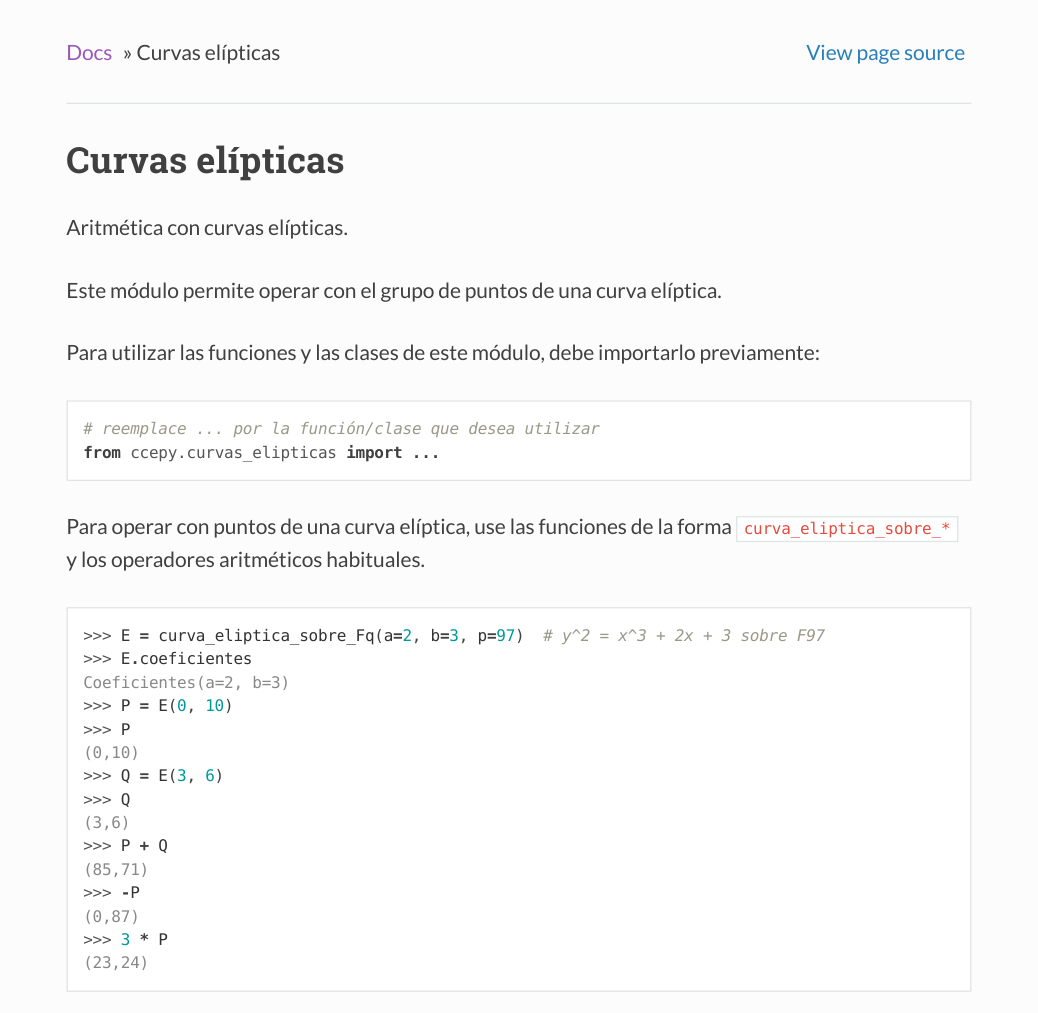
\includegraphics[scale=0.55]{Graficos/ejemplo_documentacion2}
    \caption{Captura de la documentación.}\label{fig:ejemplo_documentacion}
\end{figure}
